%!TEX root = ../NCVC2.tex

\mysection{自動輪郭処理}

\subsection{自動輪郭処理}

\begin{minipage}[t]{0.5\textwidth}
 形状認識処理ができた状態で、\menu{編集>加工指示>自動輪郭処理} を選択します
(ツールバーの Auto ボタンでもOK)。
図\ref{fig:auto.png} のようなダイアログボックスが表示されるので、必要なオフセット値を入力してください。
ここでは 0.5mm と入力します。
オフセット値を決定しOKボタンを押すと図\ref{fig:maizuru3.png} のように自動的に輪郭オフセットが計算されます。
\end{minipage}
\begin{minipage}[t]{0.5\textwidth}
\vspace*{-2zh}
\begin{figure}[H]
\centering
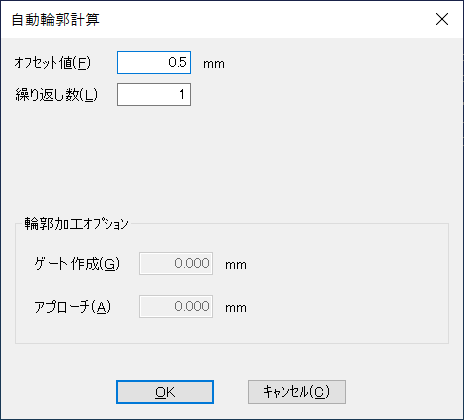
\includegraphics[scale=0.7]{No2/fig/auto.png}
\caption{サンプル図形}
\label{fig:auto.png}
\end{figure}
\end{minipage}

\begin{figure}[H]
\centering
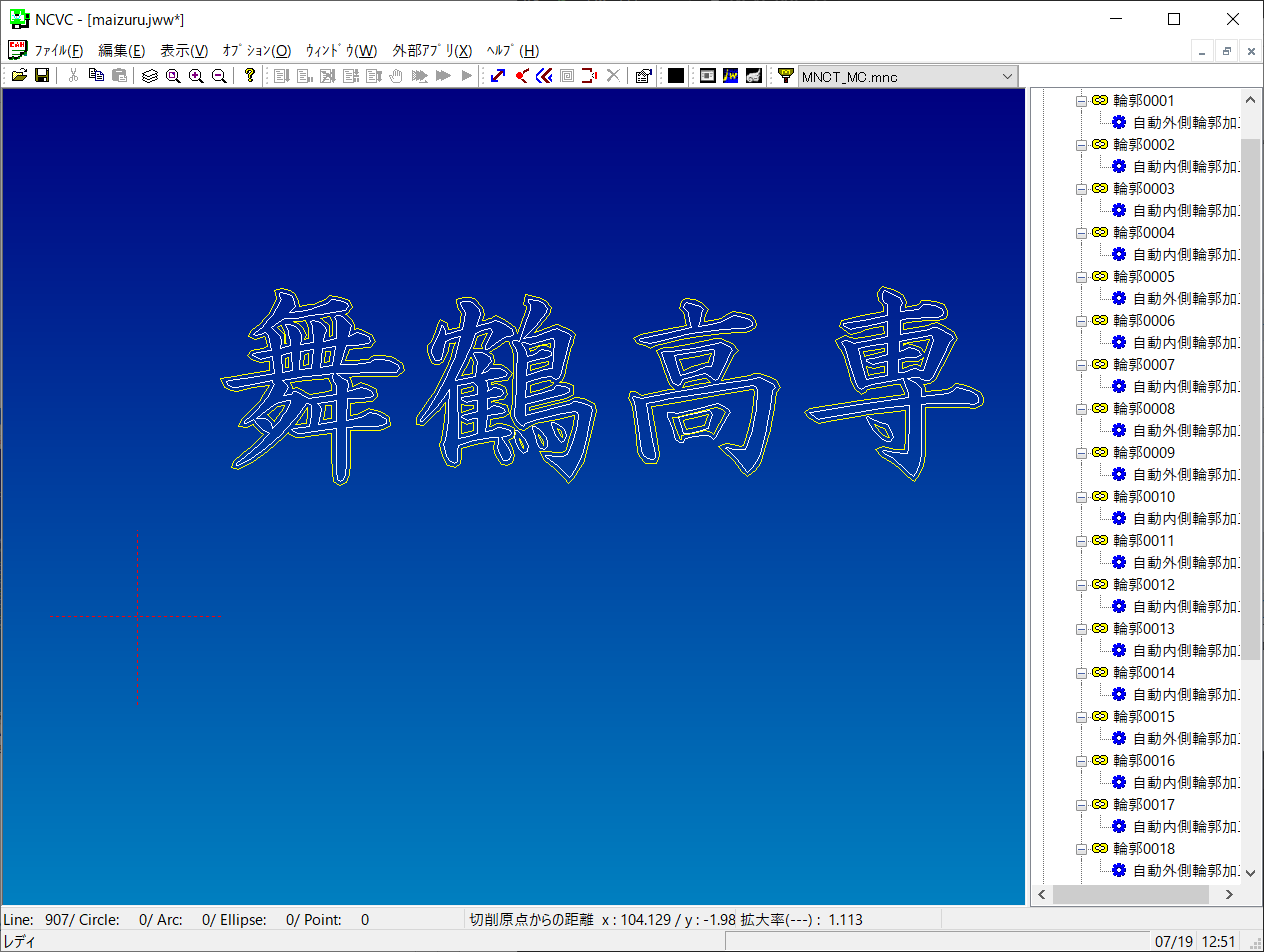
\includegraphics[scale=0.55]{No2/fig/maizuru3.png}
\caption{自動輪郭処理の結果}
\label{fig:maizuru3.png}
\end{figure}
